
%\documentclass{beamer}
\documentclass[handout]{beamer}
% This file is a solution template for:

% - Giving a talk on some subject.
% - The talk is between 15min and 45min long.
% - Style is ornate.

% Copyright 2004 by Till Tantau <tantau@users.sourceforge.net>.
%
% In principle, this file can be redistributed and/or modified under
% the terms of the GNU Public License, version 2.
%
% However, this file is supposed to be a template to be modified
% for your own needs. For this reason, if you use this file as a
% template and not specifically distribute it as part of a another
% package/program, I grant the extra permission to freely copy and
% modify this file as you see fit and even to delete this copyright
% notice. 


\mode<presentation>
{
  \usetheme{Montpellier}

  %\setbeamercovered{transparent}
  % or whatever (possibly just delete it)
}

\usepackage{xmpmulti} % package that defines \multiinclude

\usepackage[english]{babel}

\usepackage[latin1]{inputenc}

\usepackage{times}
\usepackage[T1]{fontenc}
% Or whatever. Note that the encoding and the font should match. If T1
% does not look nice, try deleting the line with the fontenc.

%\title [short title] (optional, use only with long paper titles)
\title{The Context Algorithm}

\author[Freund] % (optional, use only with lots of authors)
{Yoav Freund}
% - Give the names in the same order as the appear in the paper.
% - Use the \inst{?} command only if the authors have different
%   affiliation.

\institute[Universities of Somewhere and Elsewhere] % (optional, but mostly needed)

\subject{Machine Learning}
% This is only inserted into the PDF information catalog. Can be left
% out. 

% If you have a file called "university-logo-filename.xxx", where xxx
% is a graphic format that can be processed by latex or pdflatex,
% resp., then you can add a logo as follows:

% \pgfdeclareimage[height=0.5cm]{university-logo}{university-logo-filename}
% \logo{\pgfuseimage{university-logo}}



% Delete this, if you do not want the table of contents to pop up at
% the beginning of each subsection:
%% \AtBeginSubsection[]
%% {
%%   \begin{frame}<beamer>
%%     \frametitle{Outline}
%%     \tableofcontents[currentsection,currentsubsection]
%%   \end{frame}
%% }


% If you wish to uncover everything in a step-wise fashion, uncomment
% the following command: 

\beamerdefaultoverlayspecification{<+->}

\newcommand{\newmcommand}[2]{\newcommand{#1}{{\ifmmode {#2}\else\mbox{${#2}$}\fi}}}
\newcommand{\newmcommandi}[2]{\newcommand{#1}[1]{{\ifmmode {#2}\else\mbox{${#2}$}\fi}}}
\newcommand{\newmcommandii}[2]{\newcommand{#1}[2]{{\ifmmode {#2}\else\mbox{${#2}$}\fi}}}
\newcommand{\newmcommandiii}[2]{\newcommand{#1}[3]{{\ifmmode {#2}\else\mbox{${#2}$}\fi}}}

\newcommand{\algfnt}{\bf}

\newmcommand{\ouralg}{{\mbox{\algfnt Hedge}({\eta})}}

\newmcommand{\iter}{T}

\newfont{\cmmib}{cmmib10}
\newcommand{\boldell}{{\mbox{\cmmib \symbol{'140}}}}

\newmcommandi{\costvec}{{\boldell}^{#1}}
\newmcommandii{\cost}{{\ell}^{#1}_{#2}}

\newmcommandi{\rd}{\tilde{#1}}

\newmcommandi{\distvec}{{\bf p}^{#1}}
\newmcommandi{\rddistvec}{\rd{\bf p}^{#1}}
\newmcommandii{\dist}{{p}^{#1}_{#2}}
\newmcommandii{\rddist}{\rd{p}^{#1}_{#2}}

\newmcommandi{\bdistvec}{{\bf q}^{#1}}
\newmcommandii{\bdist}{{q}^{#1}_{#2}}

\newmcommandi{\wtvec}{{\bf w}^{#1}}
\newmcommandi{\rdwtvec}{\rd{\bf w}^{#1}}
\newmcommandii{\wt}{{w}^{#1}_{#2}}
\newmcommandii{\rdwt}{\rd{w}^{#1}_{#2}}

\newcommand{\w}[1]{\makebox[12pt]{{#1}}}
\newcommand{\Rps}{\mbox{\tt R}}
\newcommand{\rPs}{\mbox{\tt P}}
\newcommand{\rpS}{\mbox{\tt S}}
\newcommand{\rpstie}{\w{$\frac{1}{2}$}}
\newcommand{\rpswin}{\w{$0$}}
\newcommand{\rpsloss}{\w{$1$}}

\newmcommand{\decspace}{\Delta}
\newmcommand{\decsym}{\delta}
\newmcommandi{\dec}{\decsym^{#1}}
\newmcommand{\decdistsym}{\cal D}
\newmcommandi{\decdist}{{\decdistsym}^{#1}}

\newmcommand{\simpdistspace}{{\bf \cal S}}
\newmcommand{\domset}{{\rm dom}(\decdistsym)}

\newmcommand{\expdistsym}{{\cal E}}
\newmcommandii{\expdist}{{\expdistsym}^{#1}_{#2}}
\newmcommand{\expdecsym}{{\varepsilon}}
\newmcommandii{\expdec}{\expdecsym^{#1}_{#2}}

\newmcommand{\outspace}{\Omega}
\newmcommand{\outsym}{\omega}
\newmcommandi{\out}{\outsym^{#1}}

%\newmcommandii{\Dkl}{D_{\mbox{kl}}\paren{#1||#2}}
\newmcommandii{\Dkl}{{\rm {KL}}\paren{{#1}\;||\;{#2}}}

\newmcommandi{\sumwts}{\sum_{i=1}^N \wt{#1}{i}}

\newmcommand{\lossalg}{L_A}
\newmcommand{\lossouralg}{{L_{\mbox{\scriptsize\algfnt Hedge}(\eta)}}}
\newmcommand{\lossS}{{L_{\mbox{\scriptsize\algfnt S}}}}
\newmcommandi{\lossi}{L_{#1}}
\newmcommandii{\lossit}{L_{#1}^{#2}}

\newmcommandi{\upbnd}{\tilde{#1}}

\newcommand{\angles}[1]{{\left\langle {#1} \right\rangle}}
\newcommand{\paren}[1]{{\left( {#1} \right)}}
\newcommand{\abs}[1]{{\left| {#1} \right|}}
\newcommand{\ceiling}[1]{{\left\lceil {#1} \right\rceil}}

\newfont{\msym}{msbm10}
\newcommand{\real}{\mbox{\msym R}}

\newmcommand{\updatefcn}{U_\eta}

%% \newtheorem{theorem}{Theorem}	
%% \newtheorem{lemma}[theorem]{Lemma}
%% \newtheorem{corollary}[theorem]{Corollary}
%% \newtheorem{definition}{Definition}

%\newcommand{\proof}{\noindent{\bf Proof:} }
%\newcommand{\example}[1]{{\em Example #1.} }
%\newcommand{\qed}{\rule{0.7em}{0.7em}}

\newcommand{\WeakAlg}{\mbox{\algfnt WeakLearn}}
\newcommand{\Boost}{\mbox{\algfnt AdaBoost}}
\newcommand{\EX}{\mbox{\bf EX}}
\newmcommand{\hf}{h_{{f}}}
\newmcommand{\rdhf}{\rd{h}_{{f}}}
\newmcommand{\hfT}{h^T_{{f}}}
\newmcommand{\ranh}{{b}}

\newmcommand{\conclass}{{\cal C}}

\newmcommand{\badvec}{{\bf b}}
\newmcommandi{\bad}{{b}_{#1}}

%%%%%%%% New commands defined for the game-playing paper

\newmcommand{\hedge}{\algfnt Hedge}
\newmcommand{\play}{\algfnt Play}
\newmcommandi{\Glossvec}{{\bg y}^{#1}}
\newmcommandii{\Gloss}{{y}^{#1}_{#2}}
%\newmcommandi{\action}{{I}_{#1}}
\newmcommandi{\Gdistvec}{{\bf \tilde{p}}^{#1}}
\newmcommandii{\Gdist}{{\teilde{p}}^{#1}_{#2}}

%%%%%%%%%%%%%%%%%%%%%%%%%%%%%%%%%%%%%%%%%%%%%%%%%%%%%
\newmcommand{\Idistvec}{{D}}
\newmcommandi{\Idist}{\Idistvec({#1})}
\newmcommand{\Idistt}{\Idistvec_t}

\newmcommand{\Xdist}{{\cal P}}
\newmcommand{\emp}{\hat{\epsilon}}

\newmcommand{\classpc}{Y}
\newmcommand{\numclass}{k}
\newmcommandii{\prob}{\mbox{\rm Pr}_{#1}\left[{#2}\right]}
\newmcommandii{\exval}{\mbox{\rm E}_{#1}\left[{#2}\right]}

\newmcommand{\lab}{y}
\newmcommand{\ploss}{\mbox{ploss}}
\newmcommandii{\avploss}{\ploss_{#1}({#2})}
\newcommand{\sfrac}[2]{\mbox{$\frac{#1}{#2}$}}

\newcommand{\mboosta}{\mbox{\algfnt AdaBoost.M1}}
\newcommand{\mboostb}{\mbox{\algfnt AdaBoost.M2}}
\newcommand{\mboostr}{\mbox{\algfnt AdaBoost.R}}

\newmcommand{\slos}{\mbox{ploss}}
\newmcommandiii{\sloss}{\slos_{#1}({#2},{#3})}
\newmcommandiii{\avsloss}{\slos_{{#1},{#2}}({#3})}

\newmcommandii{\vwt}{{W}^{#1}_{#2}}

\newcommand{\figline}{\rule{\textwidth}{1pt}}

%\newmcommandi{\1}{{\bf 1}({#1})}
\newmcommandi{\1}{[\![{#1}]\!]}

\newmcommand{\confcn}{\kappa}
\newmcommandi{\erint}{\abs{\int_{y_i}^{h_t(x_i)} {#1} dy}}
%\newmcommandi{\erint}{\int_{\min\{y_i,h_t(x_i)\}}^{\max\{y_i,h_t(x_i)\}}{#1}dy}

\newcommand{\blue}[1]{{\color{blue}{#1}}}
\newcommand{\red}[1]{{\color{red}{#1}}}
\newcommand{\redEq}[1]{{\color{red}{$#1$}}}
\newcommand{\W}{\vec{W}}
\newcommand{\V}{\vec{V}}
\newcommand{\X}{\vec{X}}
\newcommand{\loss}{\vec{\ell}}
\newcommand{\HedgeLoss}{L_{\mbox{\footnotesize Hedge}}}


\begin{document}

%\iffalse %%%%%%%%%%%%%%%%%%%%%%%%%%%%%%%%%%%%%%%%%%%%%%%%%%%%%%%%%%%%%%%%%%

\begin{frame}
  \titlepage
\end{frame}

\begin{frame}
  \frametitle{Outline}
  \tableofcontents[pausesections]
  % You might wish to add the option [pausesections]
\end{frame}

\section{Review}

\begin{frame}
\frametitle{The online Bayes Algorithm}
\begin{itemize}
\item {\color{blue} Total loss} of expert \R{$i$}
\R{$$L_i^t = - \sum_{s=1}^{t} \log p_i^s(c^s);\;\;\; L_i^0 = 0$$}
\item {\color{blue}Weight} of expert \R{$i$}
\R{$$\wt{t}{i} = \wt{1}{i} e^{-L_i^{t-1}} = \wt{1}{i} \prod_{s=1}^{t-1} p_i^s(c^s)$$}
\item
Freedom to choose initial weights.\\
 \R{$\wt{1}{t} \geq 0$}, \R{$\sum_{i=1}^n \wt{1}{i} = 1$}
\item {\color{blue}Prediction} of algorithm \R{$A$}
\R{\[
\vp_A^t = \frac{\sum_{i=1}^N \wt{t}{i} \vp_i^t}{\sum_{i=1}^N \wt{t}{i}}
\]}
\end{itemize}
\end{frame}

\begin{frame}
\frametitle{Cumulative loss vs. Final total weight}

\onslide<1-> Total weight: \R{$W^t \doteq \sum_{i=1}^N \wt{t}{i}$}

\onslide<2-> \R{$$
\frac{W^{t+1}}{W^t}  =  \frac{\sum_{i=1}^N \wt{t}{i} e^{\log p_i^t(c^t)}}{\sum_{i=1}^N \wt{t}{i}} 
\onslide<3->          =   \frac{\sum_{i=1}^N \wt{t}{i} p_i^t(c^t)}{\sum_{i=1}^N \wt{t}{i}} 
\onslide<4->        =  p_A^t(c^t)
$$}
\onslide<5-> \R{$$ -\log \frac{W^{t+1}}{W^t} = -\log p_A^t(c^t) $$}
\R{\[
\onslide<8-> -\log W^{T+1} =
\onslide<6-> -\log \frac{W^{T+1}}{W^1} = -\sum_{t=1}^T \log p_A^t(c^t)
\onslide<7-> = L_A^T
\]}
\onslide<9-> \R{\bf EQUALITY} not bound!
\end{frame}

\begin{frame}
\frametitle{Simple Bound}
\begin{itemize}
\item Use non-uniform initial weights \R{$\sum_i \wt{1}{i} = 1$}
\item Total Weight is at least the weight of the best expert.
\R{\begin{eqnarray*}
L_A^T & = & -\log W^{T+1} 
\pause = -\log \sum_{i=1}^N \wt{T+1}{i} \\
\pause & = & -\log \sum_{i=1}^N \wt{1}{i} e^{-L_i^T} 
\pause \leq  - \log \max_i \paren{ \wt{1}{i} e^{-L_i^T} } \\
\pause & = & \min_i \paren{ L_i^T -\log \wt{1}{i} }
\end{eqnarray*}}
\end{itemize}
\end{frame}

\section{Fixed Length Markov Models}

%An Example
\begin{frame}
\frametitle{A fixed length Markov Model}
\begin{columns}
\begin{column}[t]{8cm}
\begin{itemize}
\item Observe a binary sequence.
\item \R{$x_1,\ldots,x_{t-1}$}
\item Predict next bit from past
\item \R{$P(x_t=1 | x_{t-1},x_{t-2},\ldots,x_1)$}
\item Use only last \R{$k$} bits
\item \R{$P(x_t=1 | x_{t-1},\ldots,x_{t-k})$}
\item Markov model of order \R{$k$}
\end{itemize}
\end{column}
\begin{column}[T]{5cm}
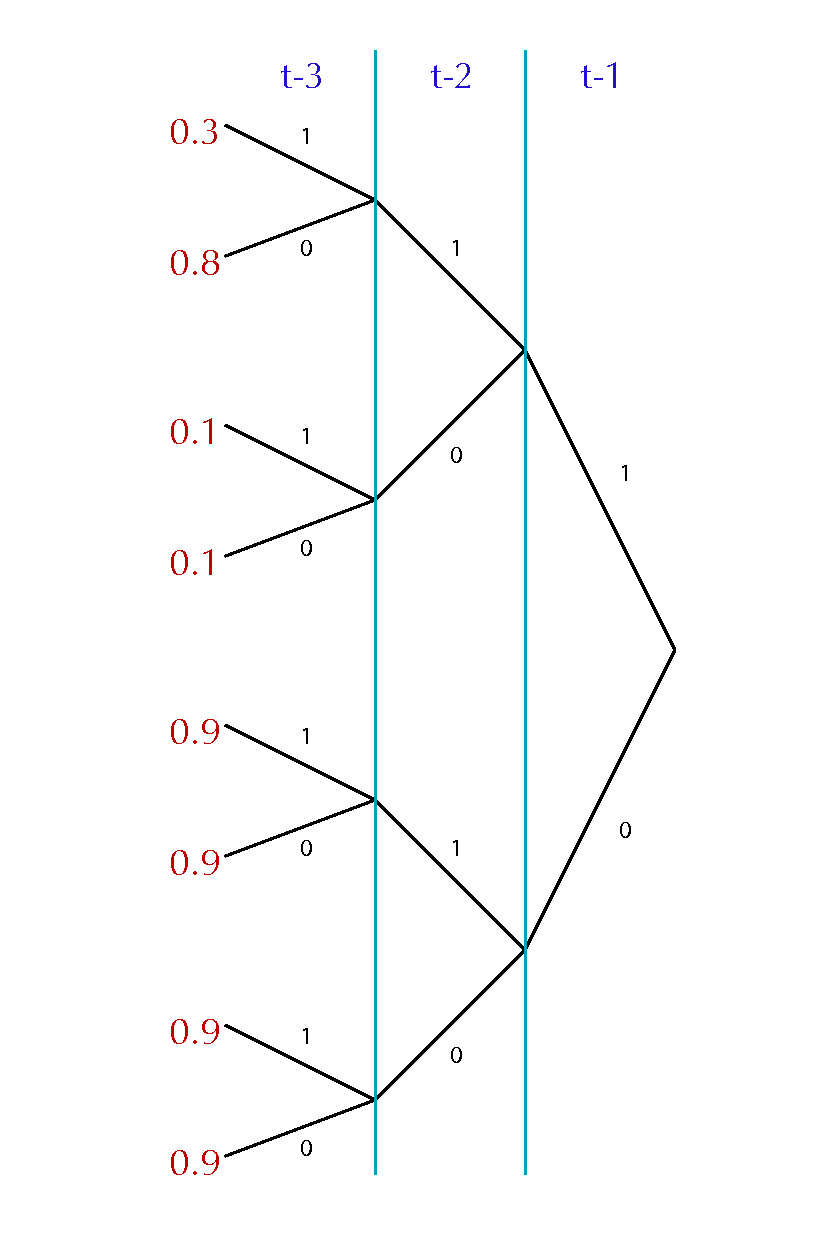
\includegraphics[width=4.5cm]{figures/PredictionTree.pdf}
\end{column}
\end{columns}
\end{frame}

%Using the KT predictor in each element
\begin{frame}
\frametitle{Learning a markov distribution}
\begin{itemize}
\item Each tree leaf is associated with a binary sequence
\R{$y_1,\ldots,y_k$} 
\item For each leaf keep two counters:
\begin{itemize}
\item \R{$a_{y_1,\ldots,y_k}$} = number of times \R{$x_{t-1}=y_1, \ldots, x_{t-k}=y_k$} \\ and \R{$x_t=0$}
\item \R{$b_{y_1,\ldots,y_k}$} = number of times \R{$x_{t-1}=y_1, \ldots, x_{t-k}=y_k$} \\ and \R{$x_t=1$}
\end{itemize}
\item Prediction (using Kritchevski Trofimov)
\R{\[p(x_t=1 | x_{t-1}=y_1,\ldots,x_{t-k}=y_k) 
= \frac{b_{y_1,\ldots,y_k}+1/2}{a_{y_1,\ldots,y_k}+b_{y_1,\ldots,y_k}+1}\]}
\item Total regret is at most \R{$2^{k-1} \log T$}
\end{itemize}
\end{frame}

\section{Variable Length Markov Model (VMM)}

%Why variable length is better than fixed length. (QU example)

\begin{frame}
\frametitle{How variable length markov can reduce regret}
\begin{columns}
\begin{column}[T]{5cm}
\multiinclude[graphics={width=4.5cm},format=pdf]{figures/PredictionTree}
\end{column}
\begin{column}[t]{8cm}
\begin{itemize}
\item Reducing number of leaves from \R{$8$} to \R{$4$} means 
\item reducing regret from \R{$4 \log T$} to \R{$2 \log T$}
\item English example: \\
\B{B \pause A \pause R \pause O \pause Q }\pause \R{U} \pause \B{E}
\item When we have little data, we can get better prediction even if the children are not 
\B{Exactly the same}
\end{itemize}
\end{column}
\end{columns}
\end{frame}

%defining complete trees
\begin{frame}
\frametitle{Prefix trees}
\begin{itemize}
\item In a prefix binary tree each node has either \R{0} or \R{2} children.
\item A node with \R{1} child means that some past histories are not covered.
\item A variable length markov model corresponds to a \B{prefix tree}.
\item But we don't know which prefix tree to use!
\end{itemize}
\end{frame}

\begin{frame}
\frametitle{Assigning probabilities to complete sequences}
\begin{itemize}
\item Using the chain rule, we can use a prediction rule to 
assign probabilities to a complete sequence.
\R{\[
P \paren{x_1=y_1,\ldots,x_T=y_T} = p \paren{x_1=y_1} p\paren{x_2=y_2|x_1=y_1} \ldots
\]}
\item
We can translate probabilities for complete sequences back into predictions.
\R{\begin{eqnarray*}
p \paren{ x_t=1 | x_1=y_1,\ldots,x_{t-1}=y_{t-1}} = \\
\frac{p\paren{x_1=y_1,\ldots,x_{t-1}=y_{t-1},x_t=1}}
{p\paren{x_1=y_1,\ldots,x_{t-1}=y_{t-1}}}
\end{eqnarray*}}
\item
Will come in handy soon!
\end{itemize}
\end{frame}

\section{Assigning weights to trees}

% Using bayesian method to perform almost as well as the best VMM
\section{Learning the structure, an inefficient solution}

\begin{frame}
\frametitle{Using online Bayes to learn the structure}
\begin{itemize}
\item We assign to each tree an initial weight of \R{$2^{-n}$} where \R{$n$} is the number of \B{nodes} in the 
prefix tree.
\item We combine the predictions of the trees using online Bayes.
\item The total regret would be \R{$\frac{l}{2}\log T + n$} where \R{$l$} is the number of \B{leaves} in the prefix tree.
\item The papers do things slightly differently because they bound the depth of the tree by \R{$k$}.
\item This algorithm maintains a weight for each tree.
\item Requires maintaining \R{$O(2^l)$} weights!
\end{itemize}
\end{frame}

% Defining the distribution using a random process.

\section{Efficient Implementation}

\begin{frame}
\frametitle{Efficient implementation}
\begin{itemize}
\item \B{First idea:} Estimate probabilities of complete sequences and use conditional to generate predictions.
\item The prior weights are used for averaging the complete sequence probabilities - they don't need to be updated.
\item \B{Second idea:} Compute the average over the prior efficiently.
\end{itemize}
\end{frame}

\begin{frame}
\frametitle{Efficient generation of prior}
\begin{itemize}
\item Prior distribution is generated by a stochastic recursion.
\item Start with root node (always exists)
\item For each node flip a fair coin.
\begin{itemize}
\item \B{Heads} Set node to be a leaf (\R{0} children)
\item \B{Tails} Create \R{2} children nodes to the node.
\end{itemize}
\item Defines a distribution over all prefix trees.
\item Probability of a tree with \R{$n$} nodes is \R{$2^{-n}$}
\end{itemize}
\end{frame}

% computing the posterior takes linear time because we can use the
% random process definition.
\begin{frame}
\frametitle{Efficient averaging over the prior (observations)}
\begin{itemize}
\item Maintain a KT estimator at each node of the tree.
\item Allocate counters only once node is visited.
\item At iteration \R{$t$} only \R{$t$} counters need to be updated.
\item Only \R{$k$} counters if depth of tree is bounded.
\item Each node is visited on a subset of the iterations.
\item Subset corresponding to node is contained in subset corresponding to node's parent.
\end{itemize}
\end{frame}

% Updating the weights takes linear time
\begin{frame}
\frametitle{Efficient averaging over the prior (procedure)}
\begin{itemize}
\item \R{$P_e\paren{a_s,b_s}$} the probability that the KT estimator at node 
\R{$s=\left\langle y_1,..,y_k \right\rangle$} assigns to it's subsequence of the past.
\item \R{$P_w^s$} the \B{average probability} assigned to the subsequence \B{over all VMM rooted} at the node \R{$s$}
\item
\R{\[
P_w^s \doteq 
\frac{P_e \paren{a_s,b_s} + P_w^{0s}P_w^{1s}}{2}
\]}
\item Average probability assigned by the complete tree is \R{$P_w^\lambda$} where \R{$\lambda$} is the root node.
\end{itemize}
\end{frame}

% Recaping the algorithm.

% generalizing the algorithm to Hedge.

% Next class thursday.

\iffalse %%%%%%%%%%%%%%%%%%%%%%%%%%%%%%%%%%%%%%%%%%%%%%%%%%%%%%%%%%%%%%%%%%
\begin{frame}
\frametitle{XXX}
\begin{itemize}
\item XXX
\end{itemize}
\end{frame}

\fi %%%%%%%%%%%%%%%%%%%%%%%%%%%%%%%%%%

\end{document}


